% Figure 2: Cohort flow and label/position distributions across splits.
% Generated by figures/make_fig2.py from FACTS.md values
% (F-COHORT-*, F-DIST-PAT-*, F-TRAIN/VAL/TEST-POSITION-DIST,
% F-SPLIT-PATIENT-OVERLAP, F-SPLIT-CENTER-SHARED).
\begin{figure}[!t]
\centering
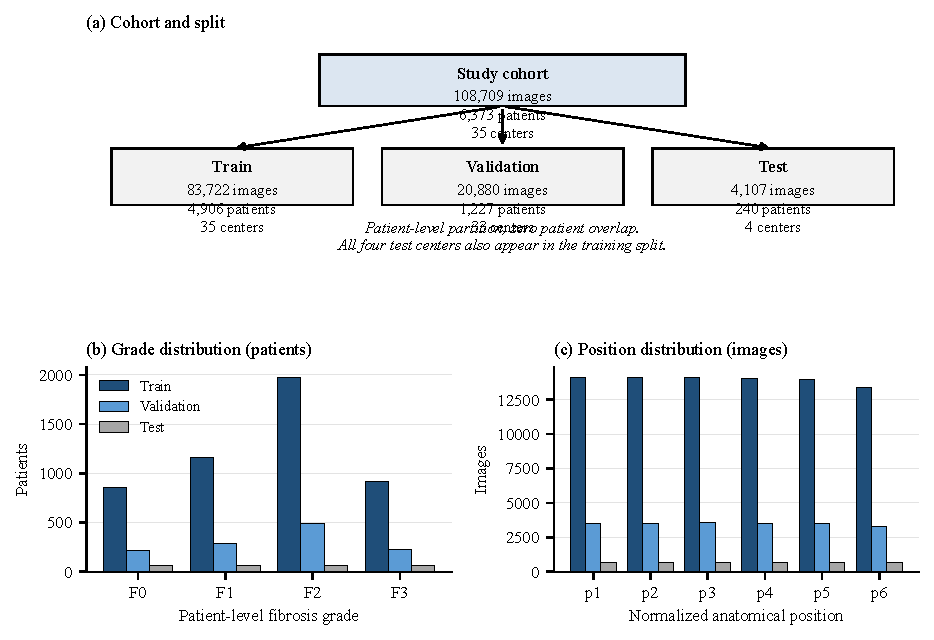
\includegraphics[width=\columnwidth]{figures/fig2_cohort.pdf}
\caption{Cohort and split characteristics. (a) The dataset is
partitioned at the patient level into training, validation and test sets with
zero patient overlap; all four centers represented in the test set also appear
in the training split. (b) Patient-level fibrosis grade distribution per split;
the test cohort contains 60 patients in each of the four stages, whereas
training and validation follow the cohort distribution. (c) Image-level counts
by normalized anatomical position (p1--p6) per split.}
\label{fig:cohort}
\end{figure}
